The interstellar medium (ISM) is the complex, continually evolving gas and dust that lies between stars.
Until recently, the study of the ISM has been limited to the Milky Way, however new technologies allow for the study of external galaxies.
In this work, the study of the ISM is restricted to that of a `disk galaxy' that comprises a thin (around 500 parsec scale height) disk of stars and an even thinner embedded disk of gaseous matter.
As an example, the stellar disk of the Milky Way has a scale height of around 400 parsecs. The gaseous matter is even more compressed, with a scale height of around 50-150 parsecs \citep{drimmel_three-dimensional_2001,kalberla_hi_2009}.

\begin{figure}
    \centering

    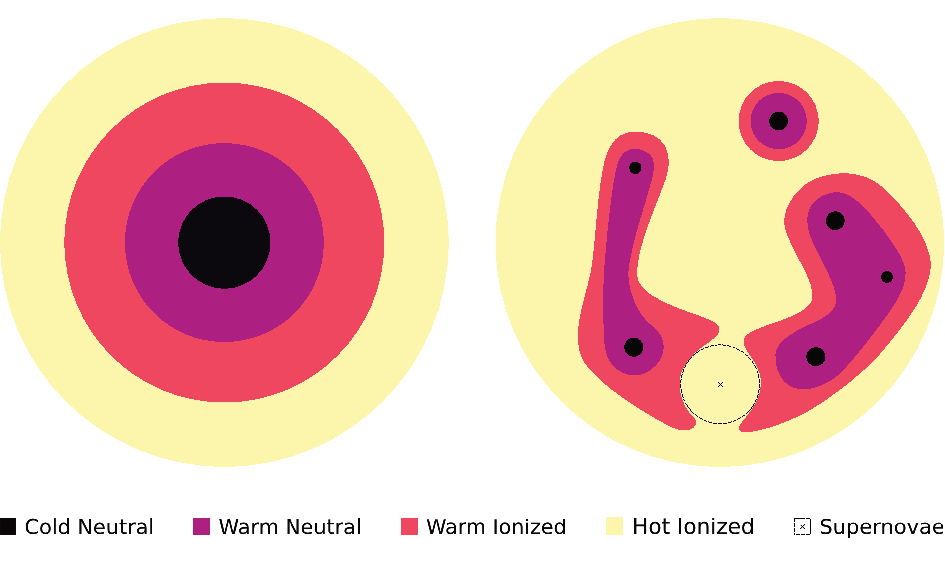
\includegraphics[width=\columnwidth]{structure_v2.pdf}

    \caption{The three-phase structure of the ISM as proposed by \citet{mckee_theory_1977}.
    On the left, the small-scale structure is shown (i.e. one cloud), whereas on the right the large-scale (a top down view of a galactic disk) is shown with multiple clouds embedded in the disk. 
    It should be noted that this figure is for illustration purposes only and does not accurately reflect the relative abundances of the phases; for a more numerical description see \citet{ferriere_interstellar_2001} and the data adapted from it in Table \ref{tab:ism}.}
    \label{fig:struct}
\end{figure}


\subsection{Three Phase Model}

The three phase model was introduced in the seminal work of \citet{mckee_theory_1977} and has since been adopted as a `standard model' of the ISM. A figure from the original work is reproduced here in Figure \ref{fig:threephase}\footnote{I intend to make my own, however here I just reproduced it} and shows how the small-scale clouds described below make up the structure of the ISM \citep{ferriere_interstellar_2001}. An overview of the properties is given in Table \ref{tab:ism}. It is worth noting that the clouds make up around $50\%$ of the total volume (and hence the vast majority of the mass) of the gaseous disk and as such their study is key to the understanding of the ISM.

\paragraph{Molecular Gas} has H$_2$ gas as its primary component and is studied through the CO radio emission that traces the gas as well as emission in the infra-red from the H$_2$ gas itself. Molecular gas forms the core of a molecular cloud and as such is shielded from the UV background produced by O and B stars, allowing it to cool to around 10 - 20 K. Because of the extremely low thermal velocities ($\approx 0.5 \mathrm{km} \mathrm{s}^{-1}$) present in this phase this region is mainly supported by turbulent motions and can undergo star formation.

\paragraph{Neutral Atomic Gas} has dissociated hydrogen (HI) as its primary component and is studied through the Ly$\alpha$ emission line and 21 cm radiation. This gas, in a similar fashion to the H$_2$ gas, is shielded from the ionizing UV background by the HII gas in the outer shell of the cloud. The neutral atomic gas is constantly heated by the inflow of heat and recombined atoms from the warm ionized gas and as such has a temperature that varies from $50$ to $10000$ K depending on the position within the cloud.

\paragraph{Warm Ionized Gas} shields the molecular and neutral gas in the cloud from the ionizing UV background produced by the O and B stars in the galaxy. This constant bombardment allows the warm ionized gas to maintain a temperature of $\approx 8000$ K and supports the emission of a radio continuum from free-free transitions. As well as the radio continuum, warm ionized gas can be studied through the use of the Balmer H$\alpha$ line.

\paragraph{Hot Ionized Gas} makes up what remains of the ISM in this model; the high temperature of the gas is due to shock-heating by supernovae. This highly ionized gas is traced by, for example, O \textsc{vi} and N \textsc{v} implying a temperature of $10^5$ K and higher with the presence of a soft x-ray background at $0.25$ keV suggesting regions with temperatures of $10^6 - 10^7$ K. 

\begin{table}
    \centering
    \resizebox{\textwidth}{!}{
        \begin{tabular}{lccc}
            Phase & $T$ (K) & $\rho$ ($n_H ~\cm^{-3}$)& Observations \\ \hline
            Molecular Gas & $10 - 20$ & $10^2 - 10^6$ & Traced by CO (radio) and IR \\
            Neutral Atomic Gas & $50 - 10000$ & $0.2 - 50$ & Ly$\alpha$ and HI 21 cm radiation \\
            Warm Ionized Gas & $\approx 8000$ & $0.2 - 0.5$ & H$\alpha$ \\
            Hot Ionized Gas & $10^5 - 10^7$ & $10^{-4} - 10^{-2}$ & X-ray and highly ionized metals\\
        \end{tabular}} % end resizebox
    \caption{Overview of the phases of gas in the ISM. Data adapted from \citet{ferriere_interstellar_2001}.}
    \label{tab:ism}
\end{table}
